\chapter{Objetivos e características}

O gerenciamento dos custos do projeto deve levar em consideração como as partes interessadas desejam que esse controle seja feito. Cada parte pode medir os custos de forma diferente.

Basicamente os custos do projeto são medidos pelos valores dos recursos necessários para se completar as atividades do projeto. Mas também se deve considerar os efeitos de decisões sobre custos recorrentes de utilização, manutenção e suporte do produto, serviço ou resultado do projeto. Por exemplo, limitar o número de testes de um produto pode aumentar seu custo de manutenção.

Os processos que fazem parte do gerenciamento dos custos, representados na Figura \ref{fig:proc:ger:custos}, podem ser resumidos em:

\begin{description}
	
	\item[\textbf{Planejar o gerenciamento dos custos}]: estabelecer políticas, procedimentos e documentação para planejar, gerenciar, gastar e controlar os custos do projeto.
	
	\item[\textbf{Estimar os custos}]: desenvolver uma aproximação dos recursos monetários necessários para completar as atividades do projeto.

	\item[\textbf{Definir o orçamento}]: agregar os custos estimados individuais das atividades ou pacotes de trabalho para estabelecer uma linha de base de custos autorizada.
	
	\item[\textbf{Controlar os custos}]: monitorar o progresso do projeto para atualizar os custos e gerenciar as mudanças feitas na linha de base do custo.	

\end{description}

\begin{figure}[!h]
	\centering
	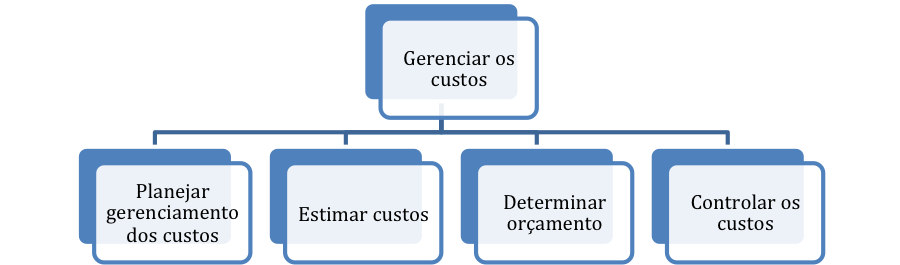
\includegraphics[scale=0.75]{Figuras/gerenciamento_custos.png}
	\caption{Processos do Gerenciamento do escopo}
	\label{fig:proc:ger:custos}
\end{figure}

\chapter{Planejar gerenciamento do custo}

O plano de gerenciamento do custo estabelece políticas, procedimentos e documentação para planejar, gerenciar, gastar e controlar os custos do projeto.

O processo de planejar o gerenciamento do custo está representado na Figura \ref{fig:custos:plan:efts} e será descrito a seguir.

\begin{figure}[!h]
	\centering
	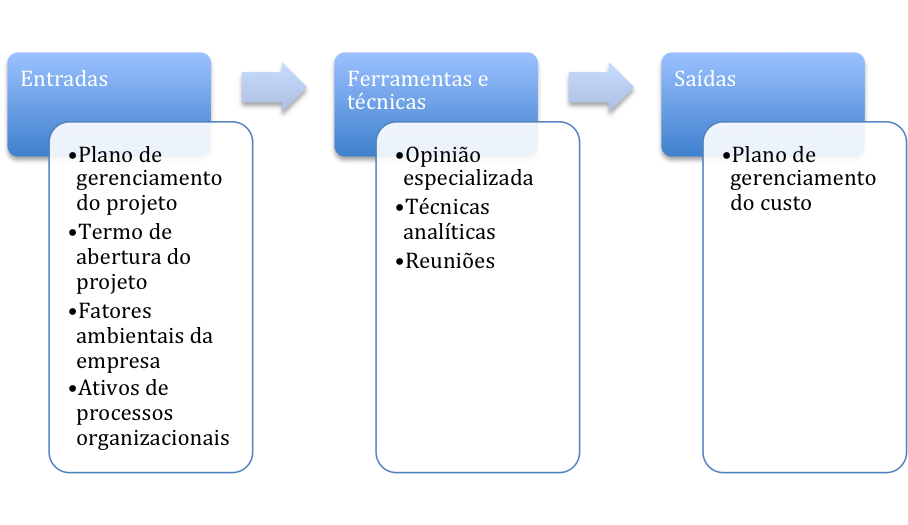
\includegraphics[scale=0.5]{Figuras/custos_efts_planejar.png}
	\caption{Planejar o gerenciamento do custo: entradas, ferramentas, técnicas e saídas}
	\label{fig:custos:plan:efts}
\end{figure}

\section{Entradas}

\begin{description}
	
	\item[Plano de gerenciamento do projeto:] contém informações importantes para se planejar o gerenciamento do custo, como a linha de base do escopo, linha de base do cronograma, entre outros.

	\item[Termo de abertura do projeto:] possui os custos em alto nível e requisitos que possam afetar o orçamento.

	\item[Fatores ambientais da empresa:] cultura, infraestrutura, condições de mercado, cotações de moedas estrangeiras, etc.

	\item[Ativos de processos organizacionais:] políticas e procedimentos internos, informações históricas, lições aprendidas, bancos de dados financeiros, etc.

\end{description}

\section{Ferramentas e técnicas}

\begin{description}

	\item[opinião especializada:] guiado por informações históricas, o especialista pode oferecer \textit{insights} valiosos sobre o ambiente e informações sobre projetos similares passados.

	\item[Técnicas analíticas:] ajudam nas decisões estratégicas sobre financiamento do projeto.
	
	\item[Reuniões:] podem participar o gerente de projetos, o patrocinador, membros selecionados da equipe, partes interessadas também selecionadas, qualquer pessoa responsável pelos custos do projeto, entre outros.
	
\end{description}

\section{Saídas}

\begin{description}
	
	\item[Plano de gerenciamento dos custos:] é um componente do \planproj e descreve como os custos serão planejados, estruturados e controlados.

\end{description}

\chapter{Estimar os custos}

Processo de desenvolver uma aproximação dos recursos monetários necessários para completar as atividades do projeto. 

O processo de estimar os custos está representado na Figura \ref{fig:custos:estimar:efts} e será descrito a seguir.

\begin{figure}[!h]
	\centering
	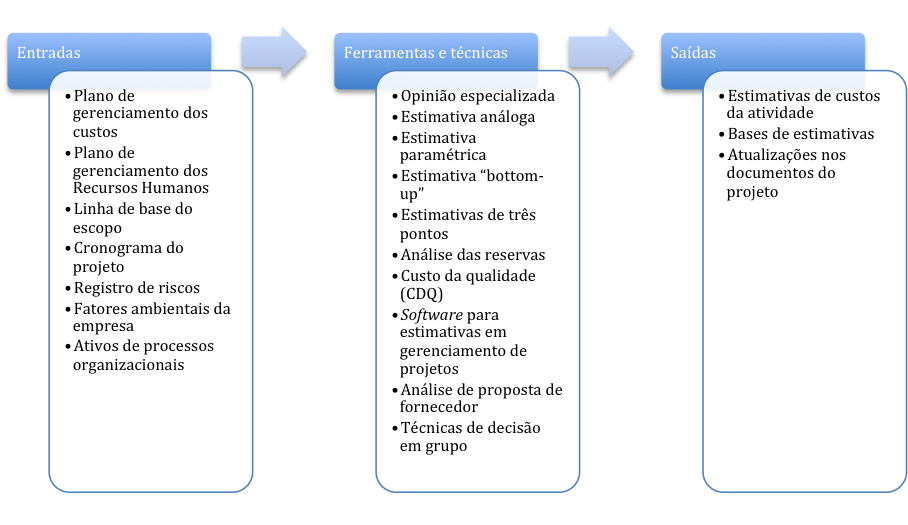
\includegraphics[scale=0.5]{Figuras/custos_efts_estimar.png}
	\caption{Estimar custos: entradas, ferramentas, técnicas e saídas}
	\label{fig:custos:estimar:efts}
\end{figure}

\section{Entradas}

\begin{description}

	\item[Plano de gerenciamento dos custos:] define comos os custos serão gerenciados e controlados.

	\item[Plano de gerenciamento dos Recursos Humanos:] oferece valores referentes aos recursos humanos que serão utilizados nas estimativas.

	\item[Linha de base do escopo:] oferece valores referentes ao produto, serviço ou resultado do projeto que serão utilizados nas estimativas.

	\item[Cronograma do projeto:] onde são encontrados a quantidade de recursos e o tempo de utilização destes recursos para estimar os custos.

	\item[Registro dos riscos:] o custo de resposta aos riscos deve ser considerado.
	
	\item[Fatores ambientais da empresa:] condições de mercado, informações comerciais publicadas, etc.
	
	\item[Ativos de processos organizacionais:] políticas de estimativa de custos, modelos de estimativas de custos, informações históricas, lições aprendidas, etc.
	
\end{description}

\section{Ferramentas e técnicas}

\begin{description}
	
	\item[Opinião especializada:] guiado por informações históricas, o especialista pode oferecer \textit{insights} valiosos sobre o ambiente e informações sobre projetos similares passados.
	
	\item[Estimativa análoga:] utiliza valores de projetos similares passados como parâmetro para estimativa dos custos.
	
	\item[Estimativa paramétrica:] utiliza relacionamento estatístico entre informações históricas relevantes e outras variáveis (por exemplo, $m^2$ construído) para calcular a estimativa de custos.
	
	\item[Estimativa \textit{bottom-up}:] custos de pacotes de trabalho individuais ou atividades são estimados e posteriormente resumidos nos níveis mais altos.
	
	\item[Estimativa de três pontos:] utiliza três estimativas:
	
		\begin{itemize}
			\item Mais provável (cM) - realista;
			\item Otimista (cO) - cenário ideal;
			\item Pessimista (cP) - pior cenário.		
		\end{itemize}
		
	As duas fórmulas mais comuns para estimativa de três pontos são:
	
		\begin{eqnarray*}
			\text{\textbf{Distribuição triangular}}&:&cE=\frac{cO+cM+cP}{3}\\	
			&&\\	
			\text{\textbf{Distribuição beta}}&:&cE=\frac{cO+4 \times cM+cP}{6}
		\end{eqnarray*}
		
	\item[Análise de reserva:] a estimativa pode incluir reservas de contingência para resposta aos riscos, cobertura de fatos desconhecidos e pode ser destinada a uma atividade específica ou para todo o projeto. Pode ser um percentual do custo estimado total, um valor fixo ou um valor determinado através de análises quantitativas.
	
	\item[Custo da Qualidade (CDQ):] podem ser utilizado para compor a estimativa.
	
	\item[\textit{Softwares} para estimativas em gerenciamento de projetos:] aplicativos, planilhas, simuladores, ferramentas estatísticas, etc.
	
	\item[Análise de proposta de fornecedor:] as estimativas podem ser feitas através da análise de propostas de fornecedores qualificados.
	
	\item[Técnicas de tomada de decisão em grupo:] auxiliam quando múltiplas alternativas forem apresentadas.
	
		
\end{description}

\section{Saídas}

\begin{description}
	
	\item[Estimativas de custos da atividade:] avaliações quantitativas dos prováveis custos necessários para executar o trabalho do projeto.
	
	\item[Bases de estimativas:] a quantia e tipo de detalhes adicionais que suportam a estimativa dos custos variam por área de aplicação. Independentemente do nível de detalhe, a documentação de suporte deve fornecer um entendimento claro e completo a respeito de como a estimativa de custos foi derivada.

	\item[Atualizações nos documentos do projeto:] registro dos riscos, entre outros.

\end{description}

\chapter{Determinar o orçamento}

Processo de agregação dos custos estimados de atividades individuais ou pacotes de trabalho para estabelecer uma linha de base dos custos autorizada. 

O processo de determinar o orçamento está representado na Figura \ref{fig:custos:orcamento:efts} e será descrito a seguir.

\begin{figure}[!h]
	\centering
	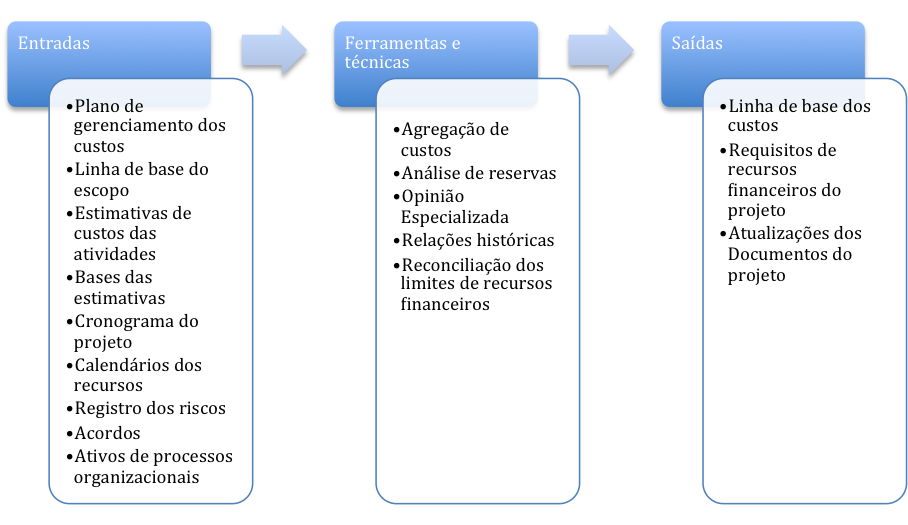
\includegraphics[scale=0.5]{Figuras/custos_efts_orcamento.png}
	\caption{Determinar o orçamento: entradas, ferramentas, técnicas e saídas}
	\label{fig:custos:orcamento:efts}
\end{figure}

\section{Entradas}

\begin{description}

	
	\item[Plano de gerenciamento dos custos:] descreve como os custos serão gerenciados e controlados.

	\item[Linha de base do escopo:] oferece informações sobre limitações, relacionamento entre pacotes de trabalho, etc.
	
	\item[Estimativas de custos das atividades:] serão agregadas para gerar as estimativas dos pacotes de trabalho.
	
	\item[Bases das estimativas:] informações adicionais sobre as estimativas.
	
	\item[Cronograma do projeto:] contém informações que podem ser usadas para agregar custos nos períodos do calendário em que os custos são planejados a incorrerem.
	
	\item[Calendários dos recursos:] contém informações que podem ser usadas para indicar os custos dos recursos durante o projeto.
	
	\item[Registro dos riscos:] deve ser revisado para considerar como os custos de resposta aos riscos serão agregados.
	
	\item[Acordos:] produtos, serviços ou outros que serão comprados durante o projeto deverão ser considerados.
	
	\item[Ativos de processos organizacionais:] políticas, procedimentos e diretrizes existentes, formais ou informais, relacionadas ao orçamento de custos, ferramentas para orçamento de custos, métodos de elaboração de relatórios, etc.
	
\end{description}

\section{Ferramentas e técnicas}

\begin{description}

	\item[Agregação de custos:] pacotes de trabalho $\rightarrow$ níveis superiores $\rightarrow$ projeto todo.
	
	\item[Análise de reservas:] reservas de contingência e reservas gerenciais.
	
	\item[Opinião Especializada:] pessoas, grupos ou empresas que possam auxiliar na determinação do orçamento.
	
	\item[Relações históricas:] quaisquer relações históricas que resultam em estimativas paramétricas ou análogas envolvem o uso de características de projetos (parâmetros) para desenvolver modelos matemáticos para prever o custo total do projeto.
	
	\item[Reconciliação dos limites de recursos financeiros:] a utilização de fundos deve ser reconciliada com quaisquer limites de recursos de fundos alocados ao projeto.
		
\end{description}

\section{Saídas}

\begin{description}
	
	\item[Linha de base dos custos:] é a versão aprovada do orçamento do projeto, sincronizado com o tempo, excluindo qualquer reserva gerencial, que só pode ser modificada através de um controle formal de mudanças e é utilizada como base de comparação com os resultados reais.
	
	\item[Requisitos de recursos financeiros do projeto:] gastos projetados mais responsabilidades antecipadas.
	
	\item[Atualizações dos Documentos do projeto:] registro dos riscos, estimativa de custos, cronograma do projeto, etc.

	
\end{description}

\chapter{Controlar os custos}

Processo de monitoramento do progresso do projeto para atualização do seu orçamento e gerenciamento das mudanças feitas na linha de base dos custos.

O processo de controlar os custos está representado na Figura \ref{fig:custos:controlar:efts} e será descrito a seguir.

\begin{figure}[!h]
	\centering
	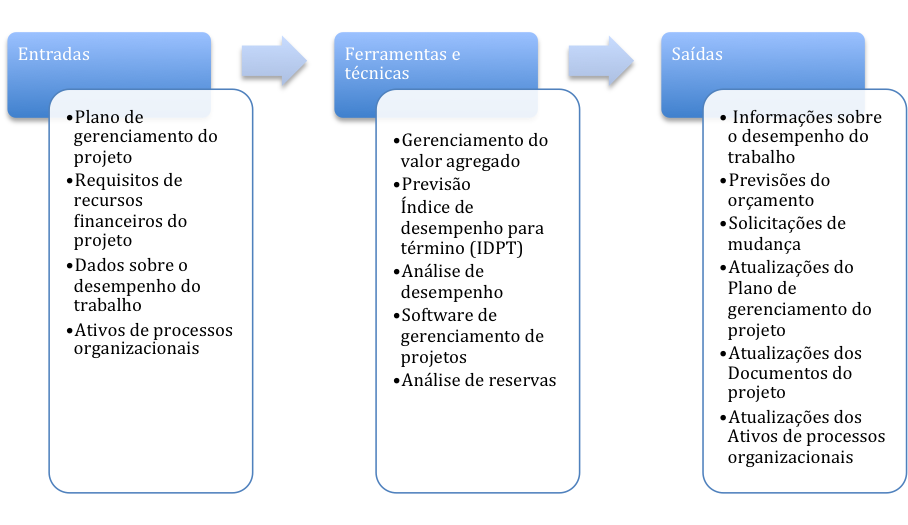
\includegraphics[scale=0.5]{Figuras/custos_efts_controlar.png}
	\caption{Controlar os custos: entradas, ferramentas, técnicas e saídas}
	\label{fig:custos:controlar:efts}
\end{figure}

\section{Entradas}

\begin{description}
	
	\item[Plano de gerenciamento do projeto:] utiliza a linha de base do desempenho de custos e o plano de gerenciamento dos custos.
	
	\item[Requisitos de recursos financeiros do projeto:] despesas do projeto e obrigações antecipadas.
	
	\item[Dados sobre o desempenho do trabalho:] custos já autorizados e incorridos.
	
	\item[Ativos de processos organizacionais:] políticas, procedimentos e diretrizes existentes, formais ou informais, relacionadas ao controle de custos, ferramentas de controle de custos e métodos de monitoramento e relato de informações a serem utilizados.
	
\end{description}

\section{Ferramentas e técnicas}

\begin{description}
	
	\item[Gerenciamento do valor agregado:] integra as medidas de escopo, custos e cronograma para auxiliar a equipe de gerenciamento a avaliar e medir o desempenho e progresso do projeto.
	
	\item[Previsão:] envolve a execução de estimativas ou prognósticos de condições e eventos no futuro do projeto com base nas informações e conhecimento disponíveis no momento da previsão.
	
	\item[Índice de desempenho para término (IDPT):] projeção calculada do desempenho de custos que deve ser atingido no trabalho restante para alcançar um objetivo de gerenciamento especificado.
	
	\item[Análise de desempenho:] compara o desempenho de custos através do tempo, atividades do cronograma ou pacotes de trabalho acima e abaixo do orçamento e recursos financeiros estimados necessários para terminar o trabalho em progresso.
	
	\item[Software de gerenciamento de projetos:] usado para monitorar os custos, mostrar tendências e prever resultados.
	
	\item[Análise de reservas:] monitorar o status das reservas de contingência e gerencial e determinar se são suficientes ou se será necessário requisitar reservas adicionais.
	
\end{description}

\section{Saídas}

\begin{description}
	
	\item[Informações sobre o desempenho do trabalho:] documentação e comunicação dos índices dos custos.
	
	\item[Previsões do orçamento:] informações sobre o orçamento são documentadas e comunicadas às partes interessadas.
	
	\item[Solicitações de mudança:] a análise do desempenho do projeto pode resultar numa solicitação de mudança da linha de base do desempenho de custos ou de outros componentes do plano de gerenciamento do projeto.
	
	\item[Atualizações do Plano de gerenciamento do projeto:] linha de base do desempenho de custos, plano de gerenciamento dos custos, etc.
	
	\item[Atualizações dos Documentos do projeto:] estimativa de custos, bases de estimativas, etc.
	
	\item[Atualizações dos Ativos de processos organizacionais:] causas de variações, ações corretivas escolhidas e suas razões, bancos de dados financeiros, lições aprendidas a partir do controle de custos, etc.
	
\end{description}